\documentclass[11pt]{article}
\usepackage[T1]{fontenc}
\usepackage{lmodern,microtype}
\usepackage[a4paper,margin=25mm]{geometry}
\usepackage{amsmath,amssymb,amsthm,mathtools}
\usepackage{graphicx,booktabs,array,longtable,enumitem}
\usepackage[numbers,sort&compress]{natbib}
\usepackage{xcolor,xurl}
\usepackage[colorlinks=true,linkcolor=blue!45!black,citecolor=blue!45!black,urlcolor=blue!45!black]{hyperref}
\newtheorem{theorem}{Theorem}[section]
\newtheorem{proposition}[theorem]{Proposition}
\newtheorem{lemma}[theorem]{Lemma}
\theoremstyle{remark}\newtheorem{remark}[theorem]{Remark}
\newcommand{\E}{\mathbb E}
\graphicspath{{../figures/}}
\setcounter{tocdepth}{1}
\hypersetup{pdftitle={The Cost of Evidence in Repeated Neural Growth},pdfauthor={Wenyu Huang}}
\title{The Cost of Evidence in Repeated Neural Growth}
\author{Wenyu Huang\\University of California San Diego}\date{}
\begin{document}
\maketitle
\begin{abstract}
Can information about what a neural network processes guide repeated
structural changes during learning? We investigate a distinction between
generating a useful operation and obtaining sufficient evidence to commit
it. A trainable shallow network repeatedly proposes an added or split unit,
fits both growth and continuation branches, and uses fresh bounded-loss
comparisons to grow, continue, or retain its current parameters. A conditional
finite-sample argument protects the entire deployed sequence, while allowing
it to remain small. The central analysis relates the evidence required for a
Brier-risk comparison to prediction movement $S$ and gain $\Delta$, with a
worst-case testing cost proportional to $S/\Delta^2$. An explicit stationary
ReLU-module sequence then separates a fresh paired-loss-only audit interface,
which requires order $K^2/D_0$ labels for $K$ powered decisions, from
precommitted shared evidence, which saves a factor $K$ up to the displayed
logarithmic terms. This is a restricted evidence-handling result, not a lower
bound for all neural learning. Ordinary-initialization experiments record
eight decisions per trajectory, compare residual, shuffled, random,
covariance, and curvature proposals, and account for rejected fits, audit
labels, and fixed-capacity alternatives. They establish repeated trained
growth in some nonlinear regimes and expose conservative stopping, proposal
attribution failures, and the value of giving fixed networks the same label
pool. A separately frozen new-seed follow-up replaces the conservative
confidence bound with an established betting test, enabling repeated growth
at the smaller audit budget while retaining finite-sample validity; random
proposals still remain competitive. The supported contribution is a theory and measurement of action
evidence, rather than a new universally effective information-growth score.
\end{abstract}
\tableofcontents

\section{The question after the earlier phases}
The original curiosity is whether information about what neural units
represent or process can guide autonomous structural adaptation. Entropy and
splitting motivate possible answers, but neither determines which operation
will improve an actual learner. We study a stationary task with a continuing
training history. The network receives repeated opportunities to change its
width, and its decisions depend on fitted candidates and observed labels.
An opportunity schedule is specified externally; growth at that opportunity
is not forced. No claim about nonstationary continual learning or semantic
specialization is made.

The preserved Phase I project concerns incompatible finite encoders under
nested refinement. It neither equates encoder states with neurons nor prices
neural optimization. Phase II separates represented information, controller
observations, and realizable splits. Its empirical advance is one structural
event with an optional heuristic holdout gate. At a designed checkpoint,
curvature helps under a short optimization budget; the advantage nearly
disappears under longer training. Its operation-aligned quantized conditional
information score has no resolved benefit in three reported tasks, while a
particular entropy proxy does help the localized task. These mixed findings
motivate independent reformulation, not a premise that information can never
help.

We ask a narrower operational question with a consequential sequence-level
implication: \emph{how does the prediction change caused by a trained action
determine the evidence needed to accept it, and what does the learner lose
by treating every structural decision as a separate audit?} A useful feature
generator and a statistically well-founded commitment rule are different
components. Either can limit progress. More information in a candidate does
not by itself prove realized benefit after decoder fitting, and a rejected
candidate does not establish that the architecture is adequate.

This phase makes four additions to the existing project. First, it implements
repeated ordinary-start neural training with growth, continuation, and
parameter retention. Second, it supplies complete sequence-valid acceptance
arguments under the implemented fresh-data protocol. Third, it gives a
quantitative movement/testing analysis and an explicit neural reset-versus-
reuse separation, including the escape that limits the lower bound. Fourth,
it performs controls that test whether proposal information adds value once
training, capacity, labels, and candidate work are visible. Theorem statements
and empirical comparisons retain their different scopes throughout.

\subsection{Independent exploration and the starting audit}
Independent investigations considered residualized features, tangent-space
deficiency, nonlinear splitting, observation limitations, audit costs, and
complementary action bundles. Residual fitting and tangent projection have
close existing formulations. The evidence-cost direction was selected because
it makes a testable prediction about an entire learning history and identifies
a resource that one-event demonstrations omit. The complementarity direction
is retained as a diagnostic boundary in Appendix~\ref{app:complementarity}.
It prevents interpreting conservative no-growth as an optimal architecture.

The workspace contains both original manuscripts, code, and raw results.
The supplied PDF hashes match the Phase III handoff exactly. Original-code
replays of five representative Phase II regimes reproduce their saved
outputs, and independent finite-difference checks confirm the relevant
training and function-preserving cloning implementation. No Phase I or II
artifact is overwritten. These are load-bearing checks, not a claim that
every inherited theorem was formally certified. The new theory does not
depend on Phase II's singular high-order split construction.

\section{Nearest results and the scope of novelty}
Cascade-Correlation already trains candidate units against residual error,
adds them progressively, and freezes their incoming weights
\cite{fahlman1990}. AdaNet explicitly compares learned subnetworks using loss
plus complexity and stops when its objective does not improve
\cite[Section 5.2, Figure 3]{cortes2017adanet}. Repeated growth and the option
to decline it are therefore not new in themselves. Our covariance control is
Cascade-inspired; it is not an exact reproduction of Cascade-Correlation's
architecture, frozen weights, or optimizer. All parameters in our grown
network remain trainable.

Splitting steepest descent derives the residual-weighted splitting matrix
and a minimum-eigenvector operation
\cite[Section 2.1, Definition 2.1]{ssd2019}. We implement that established
directional principle for Brier loss, followed by our common finite-radius
training and gate. Growing Tiny Networks defines expressivity bottlenecks by
projecting desired activity changes onto attainable directions and derives
SVD-based neuron initializations
\cite[Definition 3.1, Propositions 3.1--3.3]{verbockhaven2024growing}.
Its Appendix E.5 also explicitly accounts for controller computations.
Accordingly, a residual score or a neural growth-cost ledger cannot alone be
claimed as our novelty.

Empirical Bernstein concentration and sequential KL change of measure are
established tools \cite{maurer2009,kaufmann2016}. Adaptive evaluation has
dedicated solutions, including the Ladder leaderboard procedure
\cite{blum2015}; repeatedly consulting an ordinary holdout is not validated
merely by calling it validation. A recent representation-adequacy study
already develops sequential certification in a task-loss currency under
fixed representation and observation kernels
\cite[Section 3, Theorems 8--9]{huang2026selfcertification}; its Section 4.3 explicitly leaves
representation repair outside those guarantees. We do not claim the first
information-cost theory of representation certification.

The additional mathematical content here is the explicit movement/gain
testing specialization and a stationary neural-module sequence with a
proved separation between two evidence interfaces. The basic ingredients,
including nested Bayes projection, are credited. The neural-module theorem
does not solve general representation repair and does not apply its lower
bound to arbitrary supervised training histories. Its value is to show
precisely what must be retained or shared to avoid an otherwise repeated
evidence cost. External novelty review remains appropriate; the source audit
rules out broad originality claims without certifying worldwide priority
for the narrower composition.

% Included by main.tex. Requires amsmath, amssymb, amsthm and theorem,
% proposition, lemma, remark environments. All notation is defined locally.
\section{Prediction movement, gain, and the evidence needed to grow}
\label{sec:movement-theory}

The information used here is evidence about a proposed change in task loss.
It is not the entropy of a neuron. Two candidates can have the same small
positive gain and very different sampling difficulty, because they move
predictions by different amounts. We first make this distinction precise,
then exhibit a whole sequence for which discarding evidence between
structural decisions imposes a quadratic label cost. The latter cost is a
property of a specified audit interface; we also prove how it can be avoided.
The decomposition and statistical ingredients are classical. Our additional
result is their explicit repeated neural realization and the comparison of
fresh and shared evidence, with a deliberately bounded novelty claim.

\subsection{The geometry of a paired Brier comparison}

Let $Y\in\{0,1\}$ and $\eta(x)=\mathbb P(Y=1\mid X=x)$.
Predictions $p,q:\mathcal X\to[0,1]$ are fixed before independent audit data.
Write
\begin{equation}
 D=(Y-p(X))^2-(Y-q(X))^2,\quad h=q-p,\quad
 \Delta=\mathbb ED,\quad S=\mathbb E h^2.
 \label{eq:movement-def}
\end{equation}
Positive $\Delta$ means that $q$ improves on $p$; $S$ measures prediction
movement on population inputs.

\begin{proposition}[Movement and paired variance]
\label{prop:movement}
One has
\begin{align}
 D&=h(2Y-p-q), & \Delta&=2\mathbb E[h(\eta-p)]-S,\label{eq:gain-movement}\\
 \operatorname{Var}(D)
 &=4\mathbb E[h^2\eta(1-\eta)]
   +\operatorname{Var}\{h(2\eta-p-q)\}.\label{eq:variance-movement}
\end{align}
In particular, $|D|\le1$ and $\operatorname{Var}(D)\le4S$.
If $a\le\eta\le1-a$ almost surely, for $0<a\le1/2$, then
$\operatorname{Var}(D)\ge4a(1-a)S$.
If $p=\mathbb E[Y\mid\mathcal A]$ and
$q=\mathbb E[Y\mid\mathcal B]$ for sigma fields
$\mathcal A\subset\mathcal B$, then $\Delta=S$.
\end{proposition}
\begin{proof}
Expansion of the two squared losses gives \eqref{eq:gain-movement}.
Conditional on $X$, $h,p,q$ are constants, so
$\operatorname{Var}(D\mid X)=4h^2\eta(1-\eta)$ and
$\mathbb E[D\mid X]=h(2\eta-p-q)$.
The conditional-variance identity proves \eqref{eq:variance-movement}.
Both squared losses lie in $[0,1]$, giving $|D|\le1$; also
$|2Y-p-q|\le2$, hence $\operatorname{Var}(D)\le\mathbb ED^2\le4S$.
The noise lower bound follows from $\eta(1-\eta)\ge a(1-a)$.
Finally, $q-p$ is $\mathcal B$-measurable and
$\mathbb E[Y-q\mid\mathcal B]=0$, so
$\mathbb E[(Y-q)(q-p)]=0$. Substituting
$Y-p=(Y-q)+(q-p)$ in the difference of squared losses gives $\Delta=S$.
\end{proof}

The final assertion is the familiar projection identity for nested Bayes
refits. A trained nonlinear branch need not satisfy it. Its gain can be
small because two sizable terms in \eqref{eq:gain-movement} nearly cancel.
The ratio $S/\Delta$, when the population gain is positive, records this
discrepancy. It is a diagnostic, not a universal control objective.

\begin{proposition}[A movement-dependent sufficient audit size]
\label{prop:movement-upper}
Suppose an upper bound $S\le\bar S$ is fixed independently of the audit.
For $n$ iid paired observations and $u>0$, define
\[
 r_n=\sqrt{\frac{8\bar S u}{n}}+\frac{4u}{3n}.
\]
Each tail probability
$\mathbb P(\bar D_n-\Delta>r_n)$ and
$\mathbb P(\Delta-\bar D_n>r_n)$ is at most $e^{-u}$.
The test $\bar D_n>r_n$ therefore has false acceptance probability at most
$e^{-u}$ for $\Delta\le0$. When $\Delta>0$, the condition
\begin{equation}
 n>\max\left\{\frac{128\bar S u}{\Delta^2},
                  \frac{16u}{3\Delta}\right\}
 \label{eq:power-sample}
\end{equation}
gives power at least $1-e^{-u}$.
\end{proposition}
\begin{proof}
Put $Z=D-\Delta$ and $v=\mathbb EZ^2$. Then $|Z|\le2$.
If $v=0$, $D$ is almost surely constant and both tail bounds hold directly.
Assume henceforth $v>0$.
For $0\le\lambda<3/2$, expanding the exponential and using
$\mathbb E|Z|^k\le2^{k-2}v$ and
$k!\ge2\,3^{k-2}$ for $k\ge2$ yields
\[
 \log\mathbb Ee^{\lambda Z}
 \le\frac{\lambda^2v}{2(1-2\lambda/3)}.
\]
Apply Markov's inequality to the sum of $n$ independent copies and take
$\lambda=r/(v+2r/3)$ to obtain
\[
 \mathbb P(\bar Z_n\ge r)
 \le\exp\left\{-\frac{nr^2}{2(v+2r/3)}\right\}.
\]
For $r=\sqrt{2vu/n}+4u/(3n)$ the exponent has magnitude at least $u$.
Use $v\le4\bar S$ and repeat for $-Z$. Under
\eqref{eq:power-sample}, the square-root and linear terms of $r_n$ are
each smaller than $\Delta/4$, so $2r_n<\Delta$. Except on the lower-tail
failure event, $\bar D_n\ge\Delta-r_n>r_n$.
\end{proof}

This is a standard Bernstein argument with an explicit movement bound.
Replacing $\bar S$ by its same-sample empirical value without a confidence
bound would not satisfy the proposition. The empirical gate instead uses
an established empirical Bernstein inequality \cite{maurer2009}.
For nested Bayes refits $S=\Delta$, so the leading sufficient sample order
is $1/\Delta$; for unaligned changes it is $S/\Delta^2$.

\subsection{A matching pairwise lower-bound witness}

Write
$\operatorname{kl}(r,s)=r\log(r/s)+(1-r)\log\{(1-r)/(1-s)\}$.
For $\alpha,\beta\in(0,1)$ with $\alpha+\beta<1$, let
$b_{\alpha,\beta}=\operatorname{kl}(1-\beta,\alpha)$.

\begin{lemma}[Sequential testing, established change of measure]
\label{lem:stopped-kl}
Let $P,Q$ be finite observation laws with positive probabilities.
A randomized procedure observes iid draws, stops at a common stopping rule
$N$, and outputs an event $A$ determined by its stopped transcript.
There is no initial information whose distribution differs between the laws.
If $P(A)\ge1-\beta$ and $Q(A)\le\alpha$, then
\[
 \mathbb E_PN\,\operatorname{KL}(P,Q)\ge b_{\alpha,\beta}.
\]
\end{lemma}
\begin{proof}
If $\mathbb E_PN=\infty$ there is nothing to prove. Otherwise the stopped
log-likelihood ratio is
$L_N=\sum_{i\ge1}1_{\{N\ge i\}}\log\{P(Z_i)/Q(Z_i)\}$.
The increments are bounded, and the sum of their absolute expectations
is finite because $\mathbb E_PN<\infty$. The indicator is determined
before draw $i$, whose log-likelihood increment has mean
$\operatorname{KL}(P,Q)$. Thus
$\mathbb E_PL_N=\mathbb E_PN\operatorname{KL}(P,Q)$.
The common stopping and randomization rules contribute no extra factor
to the likelihood ratio of the stopped transcript. Its KL divergence is
therefore $\mathbb E_PL_N$. Data processing to $1_A$ bounds this below by
$\operatorname{kl}(P(A),Q(A))$.
For $r>s$, binary KL increases with $r$ and decreases with $s$, as follows
by differentiating its displayed formula. Hence this last divergence is
at least $b_{\alpha,\beta}$.
\end{proof}
The lemma is the one-observation-channel case of the established
change-of-measure result of Kaufmann, Capp\'e, and Garivier
\cite[Lemma 1 and Appendix A.1]{kaufmann2016}; its proof is included to
make the information restriction inspectable.

\begin{theorem}[A movement-dependent necessary audit size]
\label{thm:movement-lower}
For every $0<d\le1/2$ and $0<\Delta\le d/2$, there are two constant
predictions with movement $S=d^2$ and two Bernoulli label laws such that
the proposed change is risk-neutral under the first law and improves
Brier risk by $\Delta$ under the second. Any audit with false acceptance
at most $\alpha$ under the first and power at least $1-\beta$ under the
second, with no initial distinguishing information, satisfies
\[
 \mathbb E_1N\ge b_{\alpha,\beta}\frac{S}{\Delta^2}.
\]
\end{theorem}
\begin{proof}
Use a one-point input space and predictions $p=(1-d)/2$, $q=(1+d)/2$.
Let $P_0$ have label mean $1/2$ and $P_1$ mean
$1/2+\Delta/(2d)\le3/4$. Then $D=d(2Y-1)$, so the gains are zero
and $\Delta$, while $S=d^2$.
The inequality $\log u\le u-1$ applied to both Bernoulli KL terms gives
$\operatorname{kl}(r,s)\le(r-s)^2/[s(1-s)]$.
Consequently $\operatorname{KL}(P_1,P_0)\le\Delta^2/d^2$.
Lemma~\ref{lem:stopped-kl} proves the claim.
\end{proof}

This is a worst-case pair construction with fixed predictions. It does not
assert that every neural pair with the same movement and gain has this
difficulty. In particular, the gain alone gives no universal sample bound:
some restricted noiseless comparisons have deterministic positive loss
differences. Also, a gate that always rejects is safe without any samples;
the lower bound depends essentially on the stated power requirement.

\section{The cost of resetting evidence across structural decisions}
\label{sec:reset-theory}

We now give a stationary neural sequence for which the event cost is
sharp and all gains add to a fixed risk budget. This is an audit theorem
with supplied modules. It is separate from the experiments that must learn
their own candidate directions and retrain all parameters.

\subsection{Population, neural actions, and observation interface}

Fix an even $K\ge2$, $0<\varepsilon\le1/4$, and known alternating signs
$s_t=(-1)^t$. Let $X$ be uniform on $\{1,\ldots,K\}$ and
\begin{equation}
 \mathbb P(Y=1\mid X=t)=\tfrac12+s_t\theta_t,
 \qquad 0\le\theta_t\le\varepsilon.
 \label{eq:module-law}
\end{equation}
With $\rho(z)=\max\{z,0\}$, define a three-ReLU module
\begin{equation}
 \phi_t(x)=\rho(x-t+1)-2\rho(x-t)+\rho(x-t-1).
 \label{eq:relu-module}
\end{equation}
At integer inputs $\phi_t(j)=1_{\{j=t\}}$.
An installed set $A$ predicts
$f_A=1/2+\varepsilon\sum_{t\in A}s_t\phi_t$, within $[1/4,3/4]$ on the
population support. The initial predictor is $f_\varnothing=1/2$.
Each action adds three actual hidden ReLUs. Their knots and amplitude
are supplied; this construction gives no guarantee that SGD finds them.

At opportunity $t$, module $t$ is proposed, whether or not earlier modules
were accepted. The controller may retain the existing network. Its paired
loss observation is
\begin{equation}
 D_t=1_{\{X=t\}}\bigl(2s_t\varepsilon(Y-1/2)-\varepsilon^2\bigr),
 \qquad g_t=\mathbb ED_t
   =\frac{2\varepsilon\theta_t-\varepsilon^2}{K}.
 \label{eq:module-difference}
\end{equation}
These expressions are independent of earlier acceptance decisions.
The known signs are part of the supplied candidate specification. When all
$\theta_t=\varepsilon$, the Bayes prediction alternates across inputs, so
an intercept alone cannot remove the excess risk. No claim of minimal
neural width is made: the theorem fixes the local-module action family.

The \emph{fresh paired-audit interface} supplies a new iid population stream
at each opportunity and reveals only the current $D_t$.
The controller may retain all previous paired observations, decisions,
and sampling times. It does not retain labels at inputs on which the
current action makes no prediction change, nor otherwise acquire data
outside this interface. Each audit may stop sequentially using the allowed
history and environment-independent randomness. Its sample count $N_t$
includes every labelled population example drawn, including zero paired
differences. Assume the following guarantees conditional on every possible
earlier allowed transcript:
\begin{enumerate}
 \item false acceptance is at most $\alpha$ whenever $g_t\le0$;
 \item acceptance probability is at least $1-\beta$ if
 $\theta_t=\varepsilon$;
 \item the stopping rule is almost surely finite under the tested laws,
 with finite expectation under the all-positive law (otherwise the
 lower bound is immediate).
\end{enumerate}
Here $\alpha,\beta\in(0,1)$ and $\alpha+\beta<1$.
These are distribution-uniform audit requirements, not assertions about
the power of the implemented neural gate.

\begin{theorem}[Serial evidence cost and a matching audit]
\label{thm:reset-cost}
Under \eqref{eq:module-law}, take $\theta_t=\varepsilon$ for every $t$.
Every candidate has gain and movement
$\Delta_t=S_t=\varepsilon^2/K$. The initial excess Brier risk above the
Bayes predictor is $D_0=\varepsilon^2$.
Every fresh paired-audit controller satisfying the preceding requirements
obeys
\begin{equation}
 \mathbb E\sum_{t=1}^K N_t
 \ge\frac{K^2}{2\varepsilon^2}b_{\alpha,\beta}
 =\frac{K^2}{2D_0}b_{\alpha,\beta}.
 \label{eq:quadratic-reset}
\end{equation}
The expected number accepted is at least $K(1-\beta)$, and expected risk
reduction is at least $(1-\beta)D_0$.
Conversely, the same interface admits an audit satisfying these guarantees
with
\begin{equation}
 \mathbb E\sum_{t=1}^K N_t
 =K^2\left\lceil\frac8{\varepsilon^2}
       \log\frac1{\min\{\alpha,\beta\}}\right\rceil.
 \label{eq:quadratic-upper}
\end{equation}
\end{theorem}
\begin{proof}
The identity
$\mathbb E(Y-f)^2=\mathbb E[\eta(1-\eta)]+\mathbb E(\eta-f)^2$
shows that each module removes exactly $\varepsilon^2/K$ excess risk.
All $K$ remove $D_0=\varepsilon^2$; prediction movement is also
$\varepsilon^2/K$.

Fix $t$ and compare the all-positive environment $P$ to $Q_t$, which only
replaces $\theta_t$ by $\varepsilon/2$. The stage-$t$ move is risk-neutral
under $Q_t$. Every earlier observation $D_s$, $s<t$, has exactly the same
law under both environments: it is zero at $X=t$, while its only
label-dependent value occurs at $X=s$, whose label law did not change.
Inducting through the common stopping and decision rules shows that the
entire earlier allowed transcript has the same law. Conditional on almost
every transcript under this common law, no initial information
distinguishes $P$ from $Q_t$.

The signed label $\widetilde Y_t=\{1+s_t(2Y-1)\}/2$, conditional on
$X=t$, has mean $1/2+\theta_t$. Relabelling by this invertible map
preserves KL. The one-sample full-pair divergence therefore satisfies
\begin{align*}
 \operatorname{KL}(P,Q_t)
 &=\frac1K\operatorname{kl}(1/2+\varepsilon,1/2+\varepsilon/2)\\
 &\le\frac1K\frac{(\varepsilon/2)^2}
                    {(1/2+\varepsilon/2)(1/2-\varepsilon/2)}
 \le\frac{2\varepsilon^2}{K}.
\end{align*}
The last denominator is at least $15/64$; the displayed factor two is
conservative. Mapping full pairs to $D_t$ cannot increase KL.
Apply Lemma~\ref{lem:stopped-kl} conditionally on the earlier transcript
to obtain $\mathbb E_P[N_t\mid\text{history}]
\ge Kb_{\alpha,\beta}/(2\varepsilon^2)$.
Integration and summation prove \eqref{eq:quadratic-reset}.
Conditional power and linearity of expectation give the remaining
lower-bound assertions. The decisions need not be independent.

For the upper bound, let
$m=\lceil8\varepsilon^{-2}\log(1/\min\{\alpha,\beta\})\rceil$.
At stage $t$, wait for $m$ nonzero paired observations; these are exactly
the examples with $X=t$, and either nonzero value identifies $Y$.
Accept if their mean signed label $\widetilde Y_t$ exceeds
$1/2+3\varepsilon/4$.
For $\theta_t\le\varepsilon/2$ and for $\theta_t=\varepsilon$, the mean
is at least $\varepsilon/4$ from the threshold in the appropriate
direction. The Bernoulli Hoeffding bound gives either error at most
$e^{-m\varepsilon^2/8}\le\min\{\alpha,\beta\}$.
For completeness, Hoeffding's bound follows by bounding the centered
Bernoulli moment generating function by $e^{\lambda^2/8}$,
applying Markov's inequality to $m$ independent samples, and optimizing
at $\lambda=4a$ for a deviation $a$; the result is $e^{-2ma^2}$.
The waiting time to $m$ occurrences of an event of probability $1/K$ has
mean $Km$, being the sum of $m$ geometric waiting times of mean $K$.
Summing over opportunities proves \eqref{eq:quadratic-upper}.
\end{proof}

For fixed small error probabilities, the cost is quadratic in the number
of useful proposed modules at fixed total removable risk. If all $K$
decisions must be simultaneously correct with probability at least
$1-\delta$, taking $\alpha=\beta=\delta/K$ supplies that guarantee and
adds the usual logarithmic factor. The lower bound is a change-of-measure
argument over an entire stationary neural sequence, not a repeated union
bound. Its limitation is equally central: the observation interface
discards off-action information, and the modules are prescribed.

\subsection{A constructive escape through shared evidence}

\begin{theorem}[Precommitted reuse removes a factor $K$]
\label{thm:shared-evidence}
In the same population, fix all modules before seeing labels and assume
each $\theta_t$ is either at most $\varepsilon/2$ or exactly $\varepsilon$.
One common batch of
\begin{equation}
 n=\left\lceil\frac{16K}{\varepsilon^2}\log\frac{2K}{\delta}\right\rceil
 \label{eq:shared-n}
\end{equation}
iid labelled pairs is sufficient to accept every positive separated
alternative and reject every nonpositive proposed change with probability
at least $1-\delta$. The accepted modules can be installed successively.
On the subfamily $\theta_t\in\{0,\varepsilon\}$ the resulting network
contains exactly the needed modules on this event, including no growth
when all $\theta_t=0$.
\end{theorem}
\begin{proof}
For each coordinate, use its signed labels $\widetilde Y_t$ in the common
batch and accept if their mean exceeds $1/2+3\varepsilon/4$.
Let $C_t$ count examples at coordinate
$t$ and put $m_0=n/(2K)$. A multiplicative binomial bound gives
$\mathbb P(C_t<m_0)\le e^{-n/(8K)}$.
It follows directly from Markov's inequality applied to
$e^{-\lambda C_t}$: the binomial generating function is at most
$\exp\{(n/K)(e^{-\lambda}-1)\}$; taking $\lambda=\log2$ gives
an exponent no greater than $-n/(8K)$ at $C_t=n/(2K)$.
Conditional on counts and $C_t\ge m_0$, Hoeffding's bound makes the
test error at most
$e^{-m_0\varepsilon^2/8}\le\delta/(2K)$.
Also $e^{-n/(8K)}\le\delta/(2K)$ by \eqref{eq:shared-n} and
$\varepsilon\le1/4$. A union bound over the $K$ count failures and $K$
test errors proves the claim. Locality makes each comparison independent
of which other modules were installed, so sequential installation does
not change the statements being tested.
\end{proof}

The reuse theorem is valid because the local candidates and tests were
fixed independently of the labels. It does not validate arbitrary
holdout reuse after neural fitting or feedback-dependent proposal changes;
adaptive evaluation is a separate problem with established solutions and
limitations \cite{blum2015}. Alternatively, screening inputs without
requesting labels and labelling only $X=t$ reduces the separate tests to
$Km$ total labels. It still takes $K^2m$ expected input inspections unless
direct conditional input sampling is available. These resources should
not be conflated.

The exact sequence also explains why a rejected operation is not an
adequacy certificate. At $\theta_t=\varepsilon/2$, adding amplitude
$\varepsilon$ is risk-neutral, while adding amplitude $\varepsilon/2$
would improve risk. Our no-growth statement concerns a specified action
family; it certifies complete adequacy only on the subfamily
$\theta_t\in\{0,\varepsilon\}$ stated in
Theorem~\ref{thm:shared-evidence}.

\subsection{What transfers to a learned controller}

The elementary implication
\[
 \sum_{t=1}^K\Delta_t\le D_0,\quad
 \mathbb EN_t\ge c/\Delta_t
 \quad\Longrightarrow\quad
 \sum_{t=1}^K\mathbb EN_t\ge cK^2/D_0
\]
follows from Cauchy--Schwarz. The per-event premise is not automatic;
Theorem~\ref{thm:reset-cost} supplies an exact realization. For more general
comparisons, the relevant terms may be $S_t/\Delta_t^2$, and their observed
values should be reported instead of asserting a universal exponent.

There is an additional information-accounting caveat. If initial history
$H$ has different laws under the competing environments, the correct
testing constraint is
\begin{equation}
 \operatorname{KL}(P_H,Q_H)+
 \mathbb E_PN\operatorname{KL}(P,Q)
 \ge\operatorname{kl}(P(A),Q(A)),
 \label{eq:history-kl}
\end{equation}
when the new iid stream is independent of $H$ under each environment.
This follows from the KL chain rule and the proof of
Lemma~\ref{lem:stopped-kl}; history-dependent sampling replaces the second
term by a sum of conditional divergences. Initial training or retained
audit data can pay for the decision. Dropping the first term while allowing
arbitrary historical information would make a fresh-audit lower bound
false. The same labels cannot then be counted repeatedly as new purchases.

Consequently the neural experiments below test movement, realized gain,
and audit cost along ordinary trained trajectories; they are not numerical
proofs that those trajectories satisfy the local-module lower bound.
The observation distinction survives this limitation: failure to accept
can mean either an ineffective operation or inadequate evidence for a useful
one. Recording both terms is necessary to tell these explanations apart.


\section{A trainable process with repeated commitments}
\label{sec:method}
\subsection{Network, observations, and actions}
The implemented classifier is
\begin{equation}
 p_\theta(x)=\operatorname{sigmoid}\!\left(c+\sum_{j=1}^k
 a_j\tanh(w_j^\top x+b_j)\right),\qquad
 \ell_\theta(x,y)=(y-p_\theta(x))^2.
 \label{eq:network}
\end{equation}
All incoming weights, biases, outgoing weights, and the intercept are
trainable. For input dimension $d$ there are $k(d+2)+1$ parameters.
The sigmoid bounds probabilities and makes the loss lie in $[0,1]$ without
an artificial boundedness assumption or evaluation clipping. We use Brier
loss to keep the actual training objective, audit, and movement theory aligned.

The controller is centralized. It sees the fitting inputs and labels,
current predictions, residuals, and parameters. It also sees a fresh audit
block after both competing branches have been fitted. It receives no teacher
probabilities, latent task directions, or evaluator outputs. A learned
proposal adds one unit with trained incoming parameters and outgoing weight
zero. This preserves the current predictor exactly. The first gradient step
can change the new outgoing weight; subsequent steps can train its incoming
weights. Splitting instead duplicates a selected unit, halves its outgoing
weight, and perturbs the two incoming weight vectors oppositely. All
parameters subsequently train without tying. Neither action imposes nested
partitions or permanent neuron specialization.

\subsection{Proposal generation as a controlled mechanism}
For a fitting sample of size $n_F$, freeze current predictions $p_i$ and
residuals $r_i=y_i-p_i$. For a candidate $h_{w,b}(x)=\tanh(w^\top x+b)$,
define the probability tangent $z_i=p_i(1-p_i)h_{w,b}(x_i)$. The primary
score is
\begin{equation}
 J(w,b)=\frac{(n_F^{-1}\sum_i r_i z_i)^2}
                   {n_F^{-1}\sum_i z_i^2+10^{-3}}.
 \label{eq:proposal-score}
\end{equation}
It is a regularized one-direction least-squares proxy for a small logit
addition, not an exact post-training risk improvement and not mutual
information. Its denominator and the sigmoid derivative matter; the score
has no asserted scale or reparameterization invariance. Four independent
candidate units undergo 60 Adam ascent steps. The largest training score
selects one unit, and only that grown network receives the subsequent full
branch fit. We charge the optimization of all four candidate units.

The shuffled control permutes the frozen residual vector once per opportunity
and uses the same score, candidate initializations, ascent steps, and branch
training. It isolates meaningful input--residual pairing from that proposal
search workload. Random addition chooses an untrained candidate from the same
initial pool; it uses the same gate and full branch training but costs less
proposal optimization. The covariance control maximizes
$[n_F^{-1}\sum_i r_i(h_i-\bar h)]^2$; it uses the same four-candidate and
60-step machinery. Squaring the covariance has the same maximizers as its
absolute value, but our shallow architecture and all-parameter retraining
differ from full Cascade-Correlation.

The SSD control selects the lowest eigenvalue across matrices
\begin{equation}
 \widehat S_j=\frac1{n_F}\sum_i
 2(p_i-y_i)p_i(1-p_i)a_j\tanh''(w_j^\top x_i+b_j)x_ix_i^\top.
\end{equation}
The associated incoming direction gives a radius-$0.5$ symmetric split.
Biases are not perturbed initially. The empirical gate, rather than the sign
of this infinitesimal matrix alone, decides whether the finitely trained
split is retained. This is a controlled use of SSD, not a claim to reproduce
every choice in its original training procedure.

\subsection{Growth, continuation, or holding the checkpoint}
At opportunity $t$, let $I_t$ be the incumbent. Independently of the upcoming
audit, fit a same-width continuation $C_t$ and one proposed growth $G_t$ from
the same incumbent, each for 100 Adam steps on the persistent fitting data.
Optimizer moments reset to zero for both branches. After a decision, only
the selected parameters become the next incumbent. Holding retains them
exactly, so an unsuccessful branch cannot silently alter the deployed model.

On $n_A$ fresh iid audit examples compute improvements for the three ordered
pairs $(I_t,C_t)$, $(I_t,G_t)$, and $(C_t,G_t)$. For paired differences $D_i$
and sample variance $s_D^2$ with denominator $n_A-1$, define
\begin{equation}
 L(D)=\bar D-\sqrt{\frac{2s_D^2\log(2/\alpha_t)}{n_A}}
             -\frac{14\log(2/\alpha_t)}{3(n_A-1)}.
 \label{eq:eb-gate}
\end{equation}
For eight opportunities and total error $\delta=0.05$, use
$\alpha_t=\delta/(3\cdot8)$. With $\tau=0.0005$, choose
\begin{equation}
 I_{t+1}=\begin{cases}
 G_t,&L(I_t-G_t)>\tau\ \text{and}\ L(C_t-G_t)>\tau,\\
 C_t,&\text{otherwise, if }L(I_t-C_t)>0,\\
 I_t,&\text{otherwise}.
 \end{cases}
 \label{eq:decision}
\end{equation}
Here $L(A-B)$ means the lower bound applied to loss of $A$ minus loss of $B$.
The positive growth margin expresses a minimum improvement requirement; it
is not a fitted biological threshold or a monetary price.

\begin{proposition}[Conditional validity over the deployed history]
\label{prop:gate}
At each opportunity, suppose all proposal generation, branch fitting, and
choice of audit size occur before an independent iid audit block is
revealed, with each audit size at least two. Losses lie in $[0,1]$. Allocate comparison error probabilities
predictably with total at most $\delta$, over a finite or countable sequence.
Then, with probability at least $1-\delta$, every accepted continuation in
\eqref{eq:decision} has lower population risk than its incumbent, every
accepted growth improves on both incumbent and fitted continuation by more
than $\tau$, and every hold leaves population risk unchanged. Therefore the
deployed incumbent risk never increases and accepted growth improvements
sum to at most the initial risk. No power or architectural adequacy guarantee
is implied by a hold.
\end{proposition}
\begin{proof}
Condition on the complete earlier history, fitting sample, and current
proposal randomness. The three predictors are then fixed, and the new
audit remains iid. For each pair $D\in[-1,1]$, apply Theorem 4 of
Maurer and Pontil \cite{maurer2009} to $(1-D)/2\in[0,1]$.
Scaling the sample variance and mean gives exactly
$\mathbb P(L(D)>\E D\mid\text{history})\le\alpha_t$ in
\eqref{eq:eb-gate}. The three pairs may use the same block; a union bound
does not require independence among them. Conditional failure bounds,
integration over histories, and the allocated total give simultaneous
coverage at all opportunities. For a countable sequence use the increasing
union of finite failure events. On the covered event the inequalities in
\eqref{eq:decision} imply the stated risk improvements; holding preserves
the predictor. Summing nonnegative risk decrements proves the budget claim.
\end{proof}

This guarantee is per specified controller trajectory. It is not a
simultaneous guarantee across every experimental seed and method without
further allocation. It protects the accepted checkpoints, not the trial
branches, warmup, or the later ungated training diagnostic. It compares
growth with a continuation from the same incumbent, not with an independently
progressing fixed-width learner. The general fresh-data guarantee applies
to the actual sigmoid network; the stronger powered-audit lower bound in
Theorem~\ref{thm:reset-cost} does not. Our controller has historical fitting
labels and is not constrained to the theorem's paired-loss-only interface.

\section{Experiments on ordinary training histories}
\label{sec:experiments}
\subsection{Tasks, samples, and the frozen confirmation protocol}
Every main task has $X\sim N(0,I_6)$ and sampled binary labels with
$\eta(x)=0.05+0.90\operatorname{sigmoid}(g(x))$. The four functions are
\begin{align*}
 g_{\rm null}(x)&=0, &g_{\rm linear}(x)&=2x_1,\\
 g_{\rm additive}(x)&=2.5\tanh(2x_1+0.6)-2\tanh(2x_2-0.5)\\
 &\quad+1.7\tanh(2x_3+0.3)-1.5\tanh(2x_4),\\
 g_{\rm interaction}(x)&=4\tanh(2x_1)\tanh(2x_2)
                 +2\tanh(2x_3)\tanh(2x_4).
\end{align*}
These are fixed synthetic mechanism tests with nuisance coordinates, not a
broad benchmark suite. Main fitting uses 2,048 iid examples. Every network
starts at width two with incoming weights $N(0,0.7^2)$, biases
$N(0,0.15^2)$, outgoing weights $N(0,0.35^2)$, and intercept zero, followed by
200 ordinary full-batch Adam updates. All-parameter fitting uses learning
rate $0.035$; candidate ascent uses $0.04$. Adam coefficients are
$(0.9,0.999)$ with denominator constant $10^{-8}$. The same rates and steps
are applied across tasks; no designed stationary checkpoint is supplied.

Exploration used separate seeds 51000--51002 and 52000--52002. After two
pilots and code review, the method, comparison set, outcomes, and 16 new
seeds 61000--61015 were recorded before confirmation. The two main
finite-bound protocols use 4,096 and 16,384 fresh labels per opportunity at
the same fitting sample size. They share fitting data, evaluation inputs,
starting parameters, and event-indexed candidate initializations. Their
audit blocks are separate draws, not nested prefixes. Within a method,
all eight audit blocks are disjoint. No block is returned to its fitting
loop. After selection, audit outcome information enters the next incumbent,
which is why fresh data are needed for the next conditional argument.

An acceptance ablation uses the empirical means in
\eqref{eq:decision} instead of the lower bounds, with the same $\tau$, data,
and residual/shuffled/random proposal rules. It is explicitly heuristic
and has no sequence risk guarantee. It does not replace the primary method
based on favorable final evaluation. Both protocols and all unfavorable
trajectories remain in the raw files.

Evaluation averages
$(p_\theta(X)-\eta(X))^2+\eta(X)(1-\eta(X))$ over 16,384 independent inputs.
It exactly integrates conditional Bernoulli label noise but is Monte Carlo
over $X$, not exact population evaluation. These probabilities are accessed
only by evaluator functions after the action is fixed. Independent runs are
the replication unit. Reported paired intervals are two-sided 95\% Student
$t$ intervals over 16 seeds, descriptive and not multiplicity-adjusted.
Identical intervals containing zero do not establish equivalence.

\subsection{Controls and accounting}
We distinguish fitting, audit, candidate optimization, final capacity, and
post-training. The retained model has $8k+1$ parameters; the controller
holds an incumbent and fits two branches. A decision opportunity costs both
100-step branch fits even if growth is rejected, plus the candidate pool's
optimization. We record parameter--example updates as an operation proxy:
training steps times sample size times parameter count. Candidate incoming
optimization contributes $4\cdot60\cdot7n_F$ at an addition opportunity.
SSD matrix formation and eigendecomposition have a separate arithmetic proxy
$O(n_Fkd^2+kd^3)$. It is not silently combined with parameter updates.

Decision-required audit prediction work is reported separately for the three
fitted predictors. Additional forwards record prediction movement for
scientific diagnosis; elapsed controller times include that instrumentation.
They exclude final evaluation and fixed-model controls. Simultaneously running
local processes and differing linear algebra costs prevent interpreting these
times as matched-hardware efficiency. Peak process memory is not measured;
final predictor parameter count is not a claim about controller memory.

An ungated width-two learner and an ordinary fixed width-ten model receive
the nominal warmup-plus-one-branch-per-opportunity budget of 1,000 full-batch
updates. Holds discard the trial training, so this is not the number of
updates embodied in every retained path. Each also receives a
separate 600-step continuation. A retrospective fixed-final-capacity model
starts from scratch at the width reached by each adaptive run and receives
the adaptive controller's branch-and-probe update proxy. This measures
alternative optimization at matched final capacity; knowing that width in
advance is diagnostic information, so this comparator is not a deployable
automatic-width method. Both it and the grown network are then trained for
600 additional steps without gates to test whether any advantage survives
longer optimization. Those tails are outside Proposition~\ref{prop:gate}.

The low- and high-audit controllers have access to 34,816 and 133,120 labelled
examples in total, despite fitting on only 2,048. A second fixed-width control
is therefore granted the entire fitting-plus-audit label pool. It cycles
random minibatches of size 256 through that pool using persistent Adam,
learning rate $0.015$, at the normalized-residual controller's training/probe
parameter--example budget. Both width two and width ten are tested, with
actual unique labels and updates logged. This is an end-of-lifetime offline
resource-allocation comparison: it receives the full pool at the outset and
uses a different competent optimizer schedule. It shows what that label
budget can buy; it does not isolate a data-only causal effect. The first
pilot's weaker sampled-pool/reset control is retained and not passed off as
this stronger comparator.

\subsection{Measured outcomes and attribution}
The main confirmation contains 192 task--seed--protocol runs, representing
832 controller trajectories and 6,656 structural opportunities. All completed
histories pass independent reconstruction of actions, parameters, resource
counts, and terminal risks. Figures~\ref{fig:learning} and
\ref{fig:decisions} display the full opportunity sequence, including holds.
Table~\ref{tab:main-results} reports every main proposal rule, rather than
selecting the best-performing rule per task.

\begin{table}[tb]
\centering\small
\begin{tabular}{llrrrr}
\toprule
Task & Proposal & $n_A=4096$ & $n_A=16384$ & Width & Grow $\ge2$ \\
\midrule
Null & Residual & 0.2532 & 0.2532 & 2.00 & 0.00 \\
 & Shuffled & 0.2532 & 0.2532 & 2.00 & 0.00 \\
 & Random & 0.2532 & 0.2532 & 2.00 & 0.00 \\
 & Covariance & 0.2532 & 0.2532 & 2.00 & 0.00 \\
 & Ssd & 0.2532 & 0.2532 & 2.00 & 0.00 \\
\addlinespace
Linear & Residual & 0.1720 & 0.1720 & 2.00 & 0.00 \\
 & Shuffled & 0.1720 & 0.1720 & 2.00 & 0.00 \\
 & Random & 0.1720 & 0.1720 & 2.00 & 0.00 \\
 & Covariance & 0.1720 & 0.1720 & 2.00 & 0.00 \\
 & Ssd & 0.1720 & 0.1720 & 2.00 & 0.00 \\
\addlinespace
Additive & Residual & 0.1472 & 0.1395 & 3.25 & 0.56 \\
 & Shuffled & 0.1472 & 0.1427 & 2.62 & 0.19 \\
 & Random & 0.1472 & 0.1377 & 3.50 & 0.62 \\
 & Covariance & 0.1472 & 0.1409 & 3.00 & 0.44 \\
 & Ssd & 0.1472 & 0.1381 & 3.38 & 0.62 \\
\addlinespace
Interaction & Residual & 0.1754 & 0.1507 & 5.62 & 1.00 \\
 & Shuffled & 0.1749 & 0.1531 & 5.25 & 1.00 \\
 & Random & 0.1739 & 0.1475 & 5.88 & 1.00 \\
 & Covariance & 0.1759 & 0.1498 & 5.69 & 1.00 \\
 & Ssd & 0.2113 & 0.2071 & 2.69 & 0.00 \\
\addlinespace
\bottomrule
\end{tabular}
\caption{Mean final Brier risk over 16 new seeds per task. Width and fraction
with at least two accepted growth events refer to the 16,384-label audit.
Both columns fit on the same 2,048 examples and use eight fresh audit blocks.
Uncertainty for the primary paired comparisons is in
Table~\ref{tab:paired-results}; complete marginal intervals are in the CSV.}
\label{tab:main-results}
\end{table}

\begin{figure}[tb]
\centering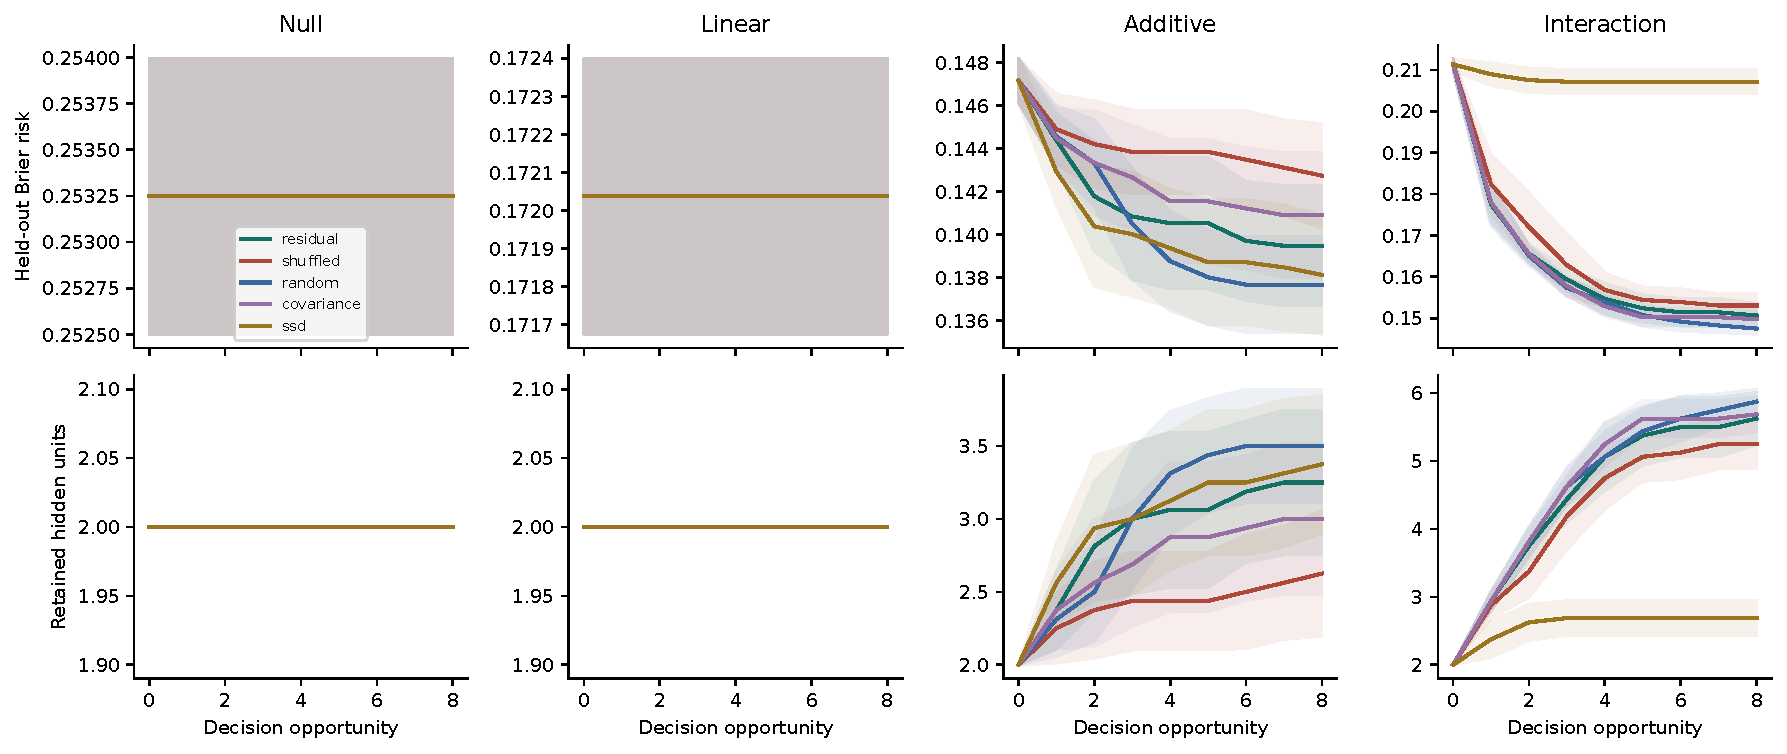
\includegraphics[width=\linewidth]{learning_trajectories.pdf}
\caption{Measured ordinary-start trajectories at 16,384 audit labels per
opportunity. Curves are mean retained risk and width; shaded bands are
pointwise 95\% Student-$t$ intervals across 16 independent seeds. Risk
integrates conditional label noise over 16,384 independent evaluation inputs.
All methods coincide on null and linear tasks. The same predictor persists
through a hold, while trial branches still consume computation.}
\label{fig:learning}
\end{figure}

\paragraph{Repeated growth and genuine no-growth.}
At the larger audit budget, the residual method accepts 20 additions across
16 additive-task runs and 58 across 16 interaction-task runs. Nine of 16
additive runs and all 16 interaction runs accept at least two additions.
Mean final widths are 3.25 and 5.625; final risks are
$0.13948\pm0.00280$ and $0.15067\pm0.00291$, where uncertainty denotes a
95\% interval half-width. Growth and holding occur within the same histories;
these are not restarts at independently constructed checkpoints. On both
null and linear tasks every primary finite-bound trajectory retains width
two and its warmup parameters. This prevents further overfitting but does
not recover Bayes risk automatically: null risk is 0.25325, above the known
0.25 Bayes risk because warmup itself was ungated.

At 4,096 audit labels, no residual additive run grows and each interaction
run grows exactly once, to width three. The interaction risk is 0.17538,
compared with 0.15067 at the larger audit budget. Fitting data and proposal
rules are fixed across this comparison, so the difference concerns the
evidence protocol and its induced history, not extra fitting samples.
It nevertheless costs four times as many audit labels. It is not a free
improvement in training efficiency.

\begin{figure}[tb]
\centering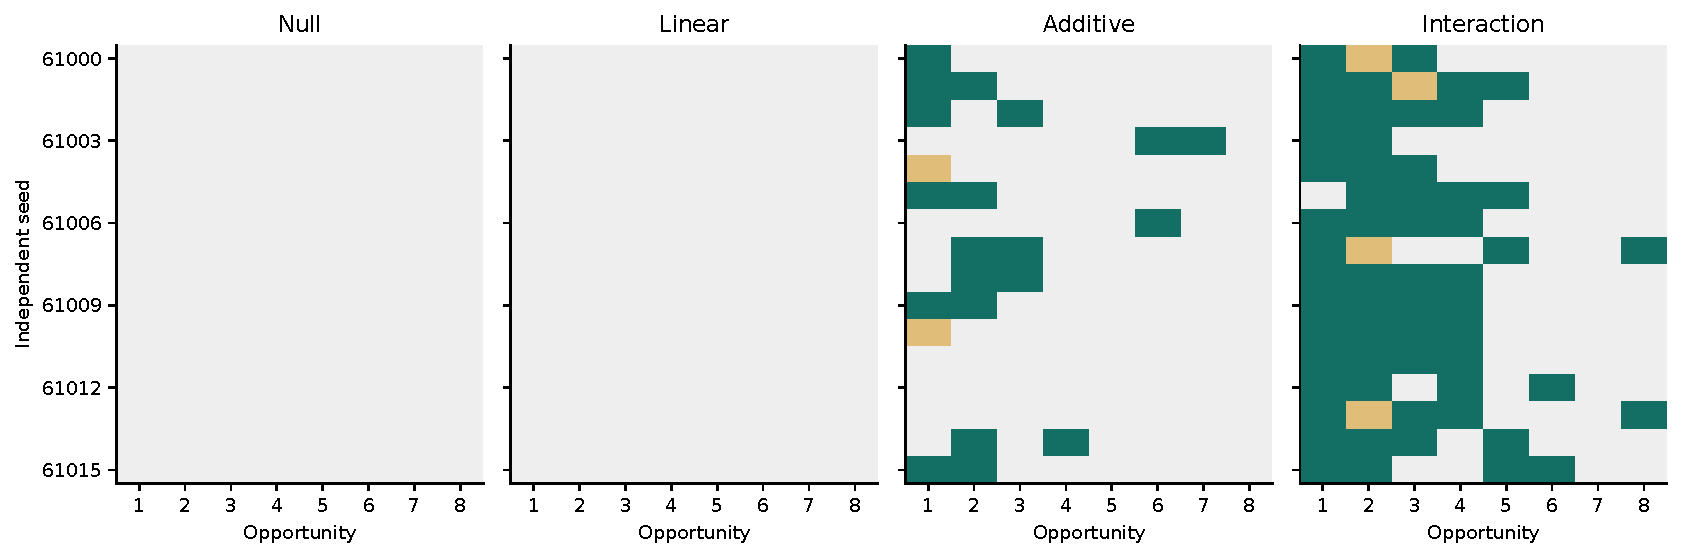
\includegraphics[width=\linewidth]{decision_histories.pdf}
\caption{Every primary residual trajectory at the larger audit budget.
Green means accepted growth; amber means accepted continuation; light gray
means the incumbent parameters are held. Rows are the 16 prespecified seeds,
columns the eight decision opportunities. An external opportunity schedule
exists, but actions and accepted final capacity are data-dependent.}
\label{fig:decisions}
\end{figure}

\paragraph{Proposal information is not a general advantage.}
Residual minus shuffled risk on the larger-audit additive task is
$-0.003268\pm0.002547$. This is a favorable comparison at equal candidate
optimization workload, with the caveat of descriptive multiple comparisons.
It does not survive the stronger interpretation of beating random proposal
addition: residual minus random is $+0.001813\pm0.002433$ on additive data
and $+0.003168\pm0.002128$ on interaction data. Random is significantly
better in the latter descriptive paired comparison while spending less on
candidate optimization. At the smaller audit budget, interaction residual
minus random is also adverse, $+0.001528\pm0.000854$.
The covariance rule is not reliably separated from the residual rule.
SSD is much worse on this interaction task, but its failure cannot establish
superiority over all growth principles: it perturbs a different restricted
action family and nearly fails to grow. These observations favor retaining
proposal alternatives instead of calling the selected residual proxy a
validated information principle.

\begin{table}[tb]
\centering\scriptsize
\begin{tabular}{lrrrr}
\toprule
Comparator & Null & Linear & Additive & Interaction \\
\midrule
shuffled & $+0.0000\pm0.0000$ & $+0.0000\pm0.0000$ & $-0.0033\pm0.0025$ & $-0.0024\pm0.0042$ \\
random & $+0.0000\pm0.0000$ & $+0.0000\pm0.0000$ & $+0.0018\pm0.0024$ & $+0.0032\pm0.0021$ \\
covariance & $+0.0000\pm0.0000$ & $+0.0000\pm0.0000$ & $-0.0014\pm0.0019$ & $+0.0009\pm0.0023$ \\
ssd & $+0.0000\pm0.0000$ & $+0.0000\pm0.0000$ & $+0.0014\pm0.0032$ & $-0.0565\pm0.0042$ \\
fixed matched & $-0.0022\pm0.0009$ & $-0.0007\pm0.0004$ & $-0.0008\pm0.0016$ & $-0.0005\pm0.0028$ \\
fixed matched tail & $-0.0007\pm0.0008$ & $-0.0004\pm0.0004$ & $-0.0008\pm0.0010$ & $-0.0023\pm0.0022$ \\
small & $-0.0016\pm0.0006$ & $-0.0001\pm0.0003$ & $-0.0066\pm0.0034$ & $-0.0595\pm0.0031$ \\
large & $-0.0229\pm0.0013$ & $-0.0176\pm0.0012$ & $-0.0120\pm0.0027$ & $-0.0067\pm0.0031$ \\
large pool & $+0.0030\pm0.0008$ & $+0.0014\pm0.0004$ & $+0.0080\pm0.0029$ & $+0.0104\pm0.0025$ \\
\bottomrule
\end{tabular}
\caption{Residual minus comparator Brier risk at the larger audit budget:
paired mean $\pm$ 95\% Student-$t$ half-width over 16 runs. Negative favors
residual growth. ``Fixed matched tail'' compares both predictors after 600
additional updates; other rows use final retained checkpoints. ``Large pool''
is width ten trained offline from the full label pool at matched training/probe
update proxy, with different minibatch optimization. Intervals are descriptive,
not multiplicity-adjusted discoveries.}
\label{tab:paired-results}
\end{table}

\begin{figure}[tb]
\centering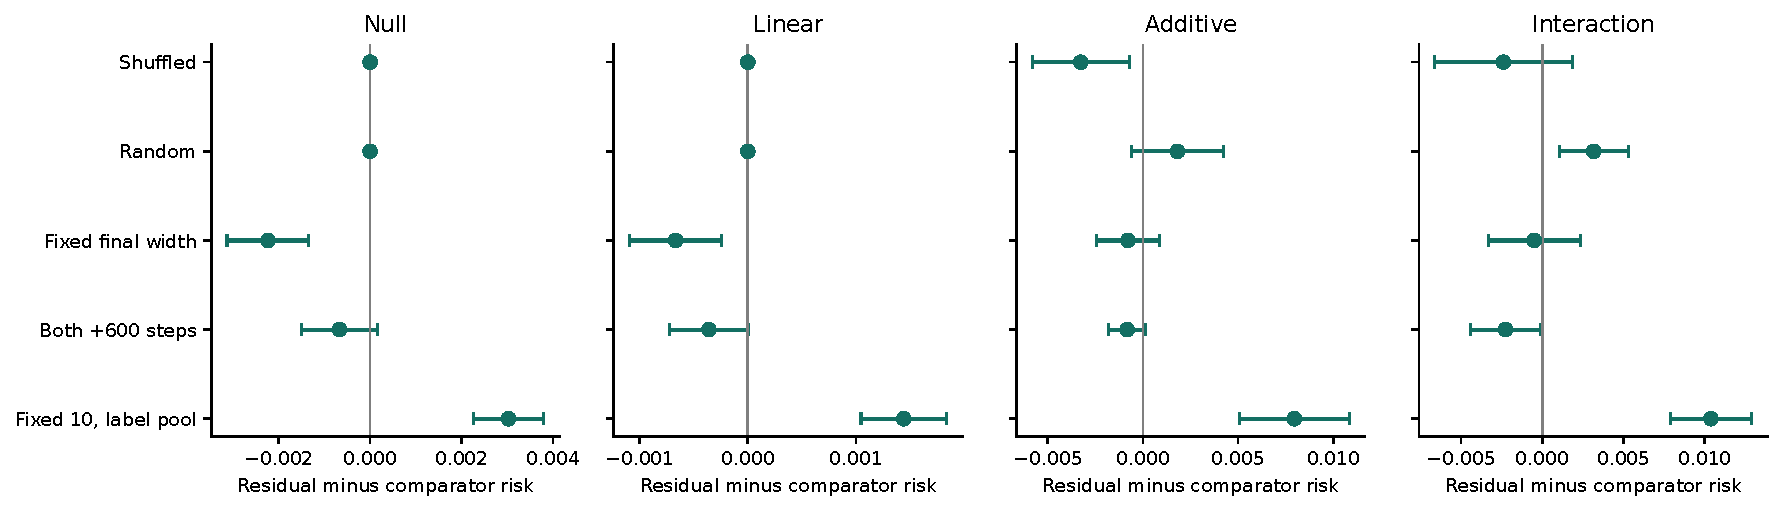
\includegraphics[width=\linewidth]{attribution.pdf}
\caption{Selected paired comparisons from Table~\ref{tab:paired-results}.
Bars are 95\% intervals across seeds. The full-label-pool comparator changes
data allocation and optimizer schedule. The two tail curves continue training
without the gate and have no risk-monotonicity guarantee.}
\label{fig:attribution}
\end{figure}

\paragraph{Capacity and optimization controls limit the attribution.}
Compared with ungated width-two training, residual growth improves mean
larger-audit risk by 0.00655 on additive data and 0.05952 on interaction data.
Thus the implemented repeated process does realize useful new capacity on
these tasks. At retrospectively matched final capacity and training/probe
work, however, paired differences are
$-0.000794\pm0.001643$ and $-0.000496\pm0.002836$: no resolved final-checkpoint
advantage. After the 600-step tail the interaction comparison is modestly
favorable, $-0.002268\pm0.002154$, while the additive interval spans zero.
This isolated tail effect does not establish a general efficiency result.
Full-batch training on 2,048 noisy labels can overfit both larger fixed
networks and grown ones. The deployed checkpoint and ungated tail therefore
must not be conflated.

At a matched training/probe update proxy, an offline width-ten learner given
the full fitting-plus-audit label pool beats the residual controller on all
four tasks. On additive and interaction data, residual minus this comparator
is $+0.007953\pm0.002875$ and $+0.010387\pm0.002514$ respectively. The
corresponding fixed-pool risks are 0.13152 and 0.14028. These models use a
different minibatch schedule and receive future audit labels at the outset;
the result is an alternative end-of-lifetime resource allocation, not a
causal estimate of the effect of labels alone. It prevents claiming a
predictive-risk advantage at this total label and training budget. The fixed
comparator deploys ten units, however, whereas the adaptive models average
3.25 and 5.625; it does not dominate them simultaneously in inference capacity.

An additional, explicitly post-hoc diagnostic addresses this capacity mismatch.
For the 64 larger-audit residual runs, a fixed learner uses the same final
width and initialization as the existing matched-width comparator, but trains
from the whole label pool with the already specified minibatch schedule and
adaptive training/probe budget. It actually consumes all 133,120 distinct
labels in every run. Residual minus this same-width pool comparator is
$+0.003111\pm0.000767$ on null data, $+0.001266\pm0.000415$ on linear data,
$+0.003491\pm0.000860$ on additive data, and
$+0.002246\pm0.001887$ on interaction data. This removes the deployed-width
mismatch and reinforces the resource-allocation limitation. The comparator
still receives labels offline, uses a different optimizer schedule, and
knows final width retrospectively. It is a diagnostic added after review,
not a preregistered primary finding or an online dominance theorem.

\begin{figure}[tb]
\centering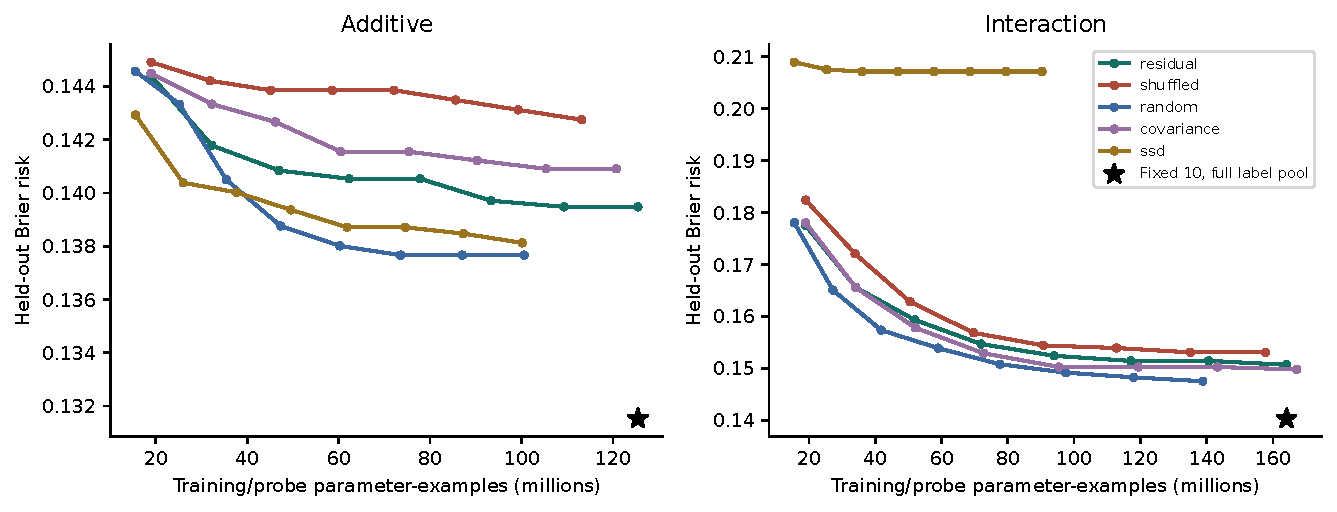
\includegraphics[width=\linewidth]{resource_trajectories.pdf}
\caption{Measured risk versus cumulative training and candidate-probe
parameter--example updates at the larger audit budget. Points summarize
16 trajectories. The fixed width-ten star uses the full label pool at the
residual controller's terminal update proxy. The horizontal axis omits audit
prediction work, matrix arithmetic, optimizer constants, and memory; these
are separately recorded and this plot is not a matched-FLOP comparison.}
\label{fig:resources}
\end{figure}

\paragraph{Rejection is partly a property of the chosen certificate.}
For the primary residual method, 253 small-audit proposals improve on both
incumbent and continuation by more than $\tau$ according to the independent
input evaluator; 237 are declined. At the larger audit size, 168 proposals
meet this evaluator criterion and 90 are declined. These counts are
diagnostic estimates, not exact population facts. The final histories differ,
so the two sets are not the same fixed proposal pool.

The smaller-audit additive task contains 125 evaluator-positive proposals,
all declined. Of these, 124 also have positive empirical cost-adjusted gains
against both comparators; 116 would fail even a bound consisting only of
the empirical-Bernstein linear term. The theoretical linear floor is
$14\log(960)/(3(n_A-1))$, approximately 0.007825 at $n_A=4096$ and
0.001956 at $n_A=16384$, before accounting for variance and the growth margin.
Consequently these failures cannot be presented as empirical confirmation
of a minimax information lower bound. They demonstrate conservatism of this
valid sufficient bound in the realized training regime.

Prediction movement and evaluator gain are separately logged for every
pair. On positive nonlinear proposals their ratios are often moderately
above the Bayes-refit identity $S=\Delta$, rather than uniformly exhibiting
extreme cancellation. Figure~\ref{fig:evidence} displays the full spread
including rejected positive proposals. A small gain alone does not diagnose
whether the proposal is weak, the empirical evidence is noisy, or the
implemented bound is unnecessarily loose.

\begin{figure}[tb]
\centering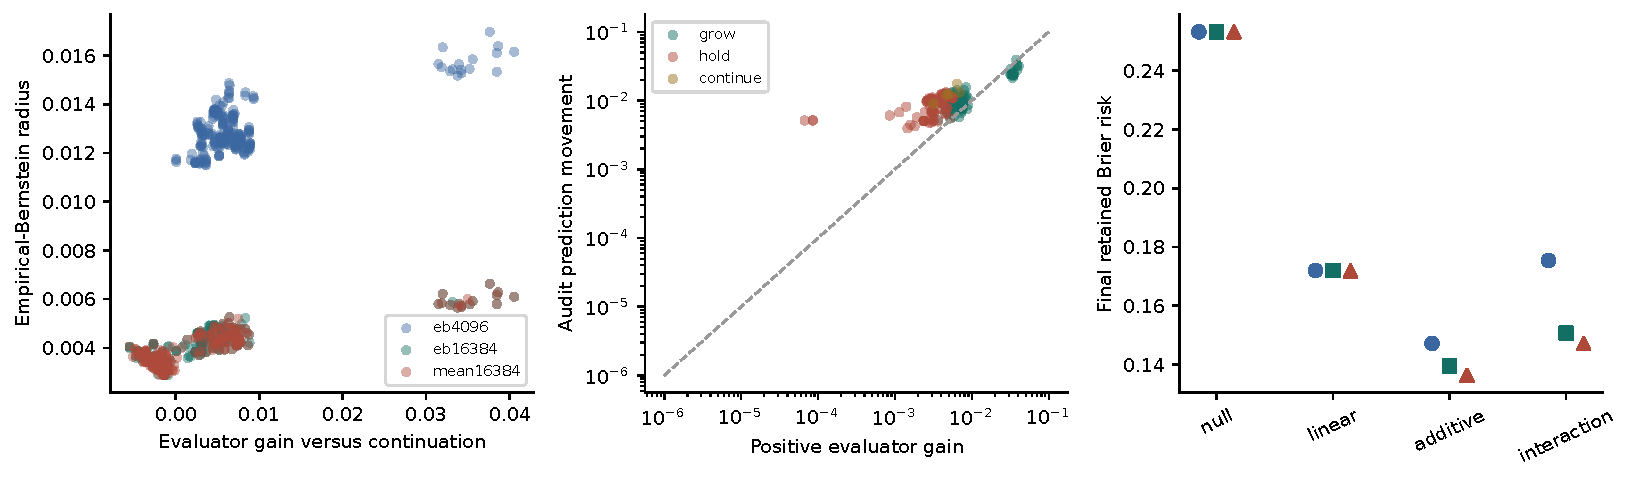
\includegraphics[width=\linewidth]{evidence_diagnostics.pdf}
\caption{Measured evidence diagnostics. Left: the finite-bound radius versus
evaluator gain over continuation for nonlinear residual proposals; the
mean-gate radius is diagnostic only. Middle: audit prediction movement versus
positive evaluator gain at the larger finite-bound audit; the dashed line is
the Bayes-refit identity, not a fitted neural law. Right: final risk under
small-audit finite bounds (blue), large-audit finite bounds (green), and the
large-audit empirical-mean heuristic (red). All input-population quantities
are Monte Carlo estimates; decisions use sampled audit labels.}
\label{fig:evidence}
\end{figure}

The heuristic mean gate accepts 97 residual growth events and reaches
mean widths 4.0625 and 6 on additive and interaction data, with risks
0.13629 and 0.14713. It provides an attainable but uncertified reference.
Twenty of its retained steps have a positive evaluator risk change, all
smaller than 0.001. No residual finite-bound retained step has an evaluator
risk increase. Neither observation replaces the population guarantee or
constitutes an exact test of its coverage; the evaluator still samples inputs.

\paragraph{The supplied-module evidence experiment.}
Separate from hidden-parameter training, 16,000 exact-distribution Monte
Carlo repetitions implement the tests in Theorems~\ref{thm:reset-cost} and
\ref{thm:shared-evidence}, with $K\in\{2,4,8,16\}$, $\varepsilon=0.2$,
and family error target 0.05. Signal, mixed, no-signal, and risk-neutral
boundary laws are retained. Negative-binomial waiting counts, multinomial
input counts, and binomial label counts are sufficient-statistic simulations
of ordinary iid sampling; they do not supply exact label expectations to
the tests. Module knots and amplitudes are nevertheless given, as stipulated
by the theorem, and no hidden parameters are trained.

At $K=16$ on the signal law, the reset procedure uses a mean 295,409 labels
versus the shared procedure's fixed 41,354, a factor 7.14 with these
conservative constants. Family correctness is 0.998 versus 1.000 over 1,000
repetitions; zero observed errors do not imply zero error probability.
At $K=2$ the shared sufficient bound costs more, 3,506 versus mean 2,952,
which is retained in the plot. Direct ReLU, Brier-risk, variance, and KL
identity checks agree to $5.6\cdot10^{-17}$. These validate the finite
realization and simulation; the lower-bound proof supplies the scaling claim.

\begin{figure}[tb]
\centering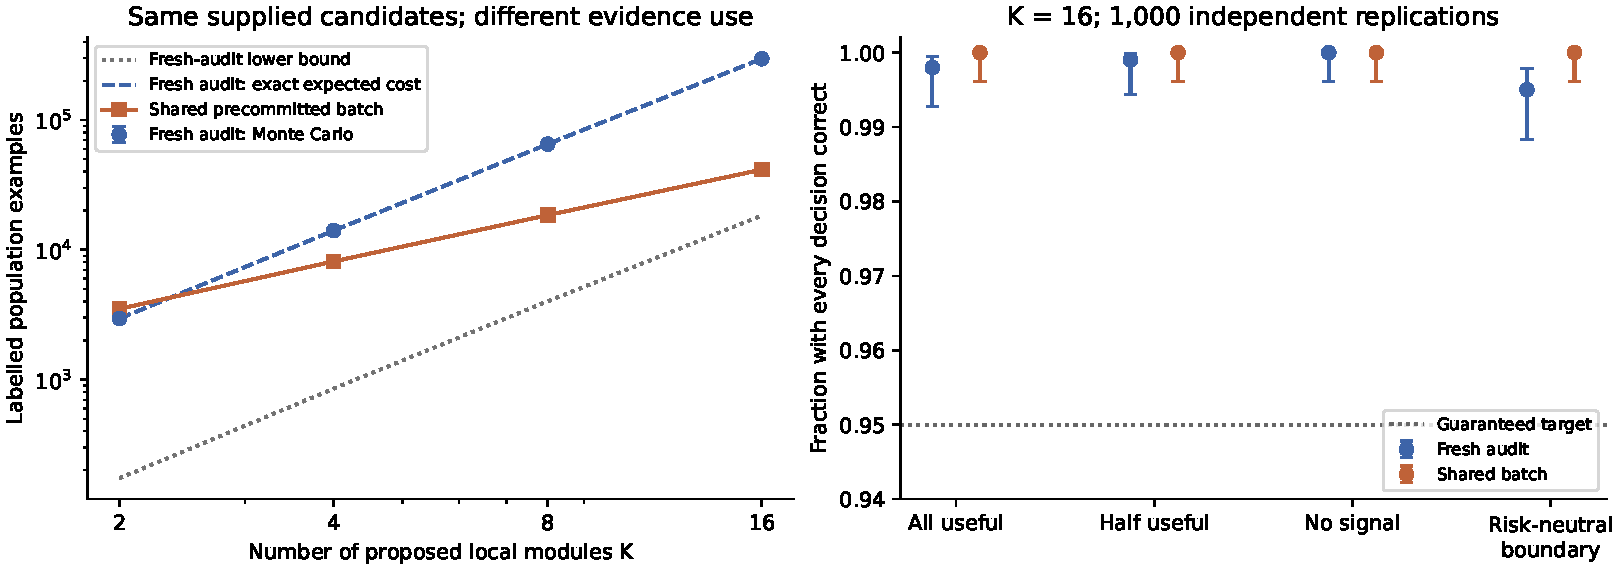
\includegraphics[width=\linewidth]{evidence_diagnostic.pdf}
\caption{Supplied-module audit experiment, not ordinary neural training.
Theoretical expected costs and lower bounds are distinguished from 1,000-run
Monte Carlo means. Error intervals retain uncertainty at zero observed
failures. The shared batch is valid because every compared local action is
precommitted, whereas the reset interface withholds off-action observations.}
\label{fig:module-evidence}
\end{figure}


\section{Constructive follow-up: improve the gate before blaming the data}
\subsection{A valid alternative to the conservative EB gate}
\label{sec:betting-gate}

The range-dependent term in the empirical Bernstein radius is a
sufficient-bound cost, which need not be unavoidable. We therefore also
test a standard bounded-mean betting construction
\cite[Section 4]{waudby2024}. This changes the evidence mechanism while
keeping proposals and training fixed; it is not a new information score
or a new statistical test.

For one comparison with required gain $\tau\in[0,1]$, put $Z_i=D_i-\tau$,
where $D_i\in[-1,1]$ is the paired Brier difference. Our implemented
thresholds are $\tau=0$ for continuation and $\tau=0.0005$ for growth.
Fix
\[
 \Lambda_\tau=\{0.05,0.1,0.2,0.5,(1+\tau)^{-1}\},\qquad
 E_n=\frac15\sum_{\lambda\in\Lambda_\tau}
          \prod_{i=1}^n(1+\lambda Z_i).
\]
For these thresholds every $\lambda\in\Lambda_\tau$ belongs to
$[0,(1+\tau)^{-1}]$. The gate accepts when $E_n\ge1/\alpha_\mathrm{pair}$.
It computes each product in logarithms and combines them by log-sum-exp;
zero factors give a zero product. The average over the five fixed values
is essential: selecting the best product without its mixture penalty
would not have this validity statement.

\begin{proposition}[Conditional validity of the implemented betting gate]
\label{prop:betting-gate}
For the implemented thresholds $\tau\in\{0,0.0005\}$,
conditional on an arbitrary training and decision history $H$, suppose
the compared predictions and $\tau$ are fixed, the audit observations
are iid, and $\mathbb E[D_i\mid H]\le\tau$. Then
$\mathbb P(E_n\ge1/\alpha_\mathrm{pair}\mid H)
\le\alpha_\mathrm{pair}$. The same bound holds for crossing the threshold
at any audit sample size, provided the prediction pair stays fixed.
Allocation $\alpha_\mathrm{pair}=0.05/(3\cdot8)$ gives probability at
most $0.05$ of any false accepted inequality during the eight-opportunity,
three-comparison implemented controller, with fresh audit data at each
opportunity.
\end{proposition}
\begin{proof}
Write $M_{\lambda,0}=1$ and
$M_{\lambda,k}=\prod_{i=1}^k(1+\lambda Z_i)$.
Since $Z_i\ge-1-\tau$ and
$0\le\lambda\le(1+\tau)^{-1}$, every factor is nonnegative.
Conditional on $H$ and the first $k-1$ audit observations,
\[
 \mathbb E[M_{\lambda,k}\mid H,Z_1,\ldots,Z_{k-1}]
 =M_{\lambda,k-1}(1+\lambda\mathbb E[Z_k\mid H])
 \le M_{\lambda,k-1}.
\]
Thus each product and their fixed average form nonnegative
supermartingales, with initial value one. In particular
$\mathbb E[E_n\mid H]\le1$, and Markov's inequality proves the
fixed-size claim. For the threshold-crossing claim, let $T$ be the first
crossing. For every finite $m$, the stopped average $E_{T\wedge m}$ has
expectation at most one: this follows by summing its conditional
nonpositive increments up to the bounded stopping time. On $\{T\le m\}$
it is at least $1/\alpha_\mathrm{pair}$, so
$\mathbb P(T\le m\mid H)\le\alpha_\mathrm{pair}$.
Let $m\to\infty$. Finally integrate the conditional comparison bounds
over $H$ and sum them over the 24 possible tests. The three comparisons
may share the current audit sample; their independence is not needed.
\end{proof}

The proposition guarantees accepted inequalities, not the discovery of
useful candidates or high power. Products are restarted for each new
prediction pair. Reusing a product after a feedback-dependent change in
the prediction pair is outside this implementation and proof. The gate
adds $15n$ factor evaluations across the three comparisons per opportunity,
in addition to the branch fitting and prediction evaluations shared with
the EB procedure. The follow-up reports these extra operations.

\subsection{Fresh-seed comparison at the smaller audit budget}
After the original confirmation exposed the empirical-Bernstein linear floor,
we froze a separate protocol before running seeds 63000--63015. Both the
betting and original EB gates use the same ordinary starts, fitting data,
fresh 4,096-label audit blocks, residual/random candidate proposals, and
branch training. This adds 128 task--seed--gate configurations, 256 controller
trajectories, and 2,048 opportunities. It is a new-seed follow-up motivated by
an earlier finding, not a retroactive change to the original confirmation.
The first experiment runner and all original results remain unchanged.

\begin{table}[tb]
\centering\scriptsize
\resizebox{\linewidth}{!}{\begin{tabular}{llrrrr}
\toprule
Task & Proposal & EB risk & Betting risk & Paired difference [95\% CI] & Width (EB / bet)\\
\midrule
null & residual & 0.25312 & 0.25312 & +0.00000 [+0.00000, +0.00000] & 2.00 / 2.00\\
null & random & 0.25312 & 0.25312 & +0.00000 [+0.00000, +0.00000] & 2.00 / 2.00\\
linear & residual & 0.17210 & 0.17210 & +0.00000 [+0.00000, +0.00000] & 2.00 / 2.00\\
linear & random & 0.17210 & 0.17210 & +0.00000 [+0.00000, +0.00000] & 2.00 / 2.00\\
additive & residual & 0.14698 & 0.13836 & -0.00861 [-0.01078, -0.00644] & 2.00 / 3.44\\
additive & random & 0.14698 & 0.13915 & -0.00782 [-0.01068, -0.00496] & 2.00 / 3.25\\
interaction & residual & 0.17558 & 0.15209 & -0.02349 [-0.02628, -0.02070] & 3.00 / 5.31\\
interaction & random & 0.17357 & 0.14955 & -0.02403 [-0.02629, -0.02177] & 3.00 / 5.56\\
\bottomrule
\end{tabular}
}
\caption{New-seed gate comparison, 16 paired repetitions per task and proposal.
Both gates use 4,096 fresh audit labels per opportunity. Paired difference is
betting minus EB Brier risk, with a descriptive 95\% Student-$t$ interval.
Width is the mean final hidden-unit count. The betting gate's extra products
are not included in training parameter--example matching.}
\label{tab:betting}
\end{table}

The alternative gate provides a substantial constructive improvement for
both proposal mechanisms. For the residual method, additive risk decreases
from 0.14698 under EB to 0.13836 under betting, a paired change of
$-0.00861$ with interval $[-0.01078,-0.00644]$. Interaction risk decreases
from 0.17558 to 0.15209, a paired change of $-0.02349$ with interval
$[-0.02628,-0.02070]$. Mean widths increase from 2 to 3.4375 on additive
data and from 3 to 5.3125 on interaction data. Null and linear networks
remain at width two with identical predictions under both gates.
These are repeated trained histories with a finite-sample commitment
guarantee, rather than forced-growth examples.

The improvement is at the same audit-label budget, not the same final
training effort. Accepted wider models require more later branch training:
residual training/probe parameter--example work rises by factors 1.206 and
1.224 on additive and interaction data. The betting calculations add
$15\cdot4096\cdot8=491{,}520$ factor evaluations per trajectory, including
rejected comparisons. Current research instrumentation also computes EB
statistics in both arms. Both consume 32,768 audit labels plus 2,048 fitting
labels; no evidence-sharing gain from Theorem~\ref{thm:shared-evidence} is
claimed for this restarted testing procedure.

The follow-up also sharpens the adverse selector evidence. Under the betting
gate, residual minus random is $-0.000789$ with interval
$[-0.003284,0.001705]$ on additive data and $+0.002542$ with interval
$[0.000242,0.004841]$ on interaction data. Random thus retains a favorable
interaction result while avoiding candidate optimization. Comparisons of
the residual method with its retrospectively matched fixed capacity and
training/probe budget remain unresolved on both nonlinear tasks. The random
betting method has a modest favorable additive comparison against its own
matched fixed model, $-0.00194$ with interval $[-0.00353,-0.00035]$; that
positive control result is retained. Larger full-label-pool networks still
have lower mean risks, with the capacity and offline-optimization caveats
described earlier.

Independent checks reconstruct all 1,024 betting-arm opportunities and
3,072 product tests from saved parameters and regenerated audit examples;
maximum log-e discrepancy is $4.0\cdot10^{-13}$. Finite-binomial null
calculations check the expectation and tail bound directly. No betting-arm
retained step increases evaluator risk in this follow-up, but that finite
observation is not the proof of validity. The proof is
Proposition~\ref{prop:betting-gate}, and evaluation remains Monte Carlo in
the input distribution.

\begin{figure}[tb]
\centering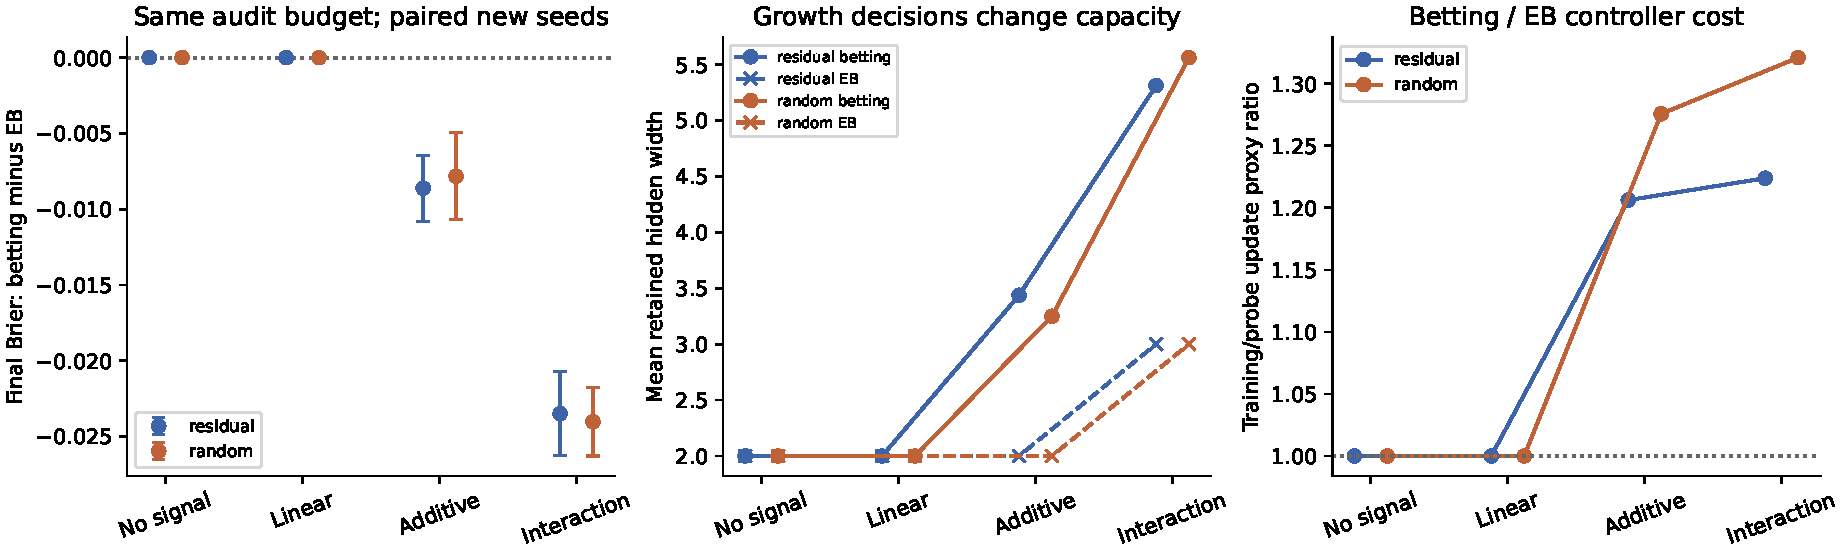
\includegraphics[width=\linewidth]{betting_followup.pdf}
\caption{Measured, fresh-seed gate follow-up at the same smaller audit budget.
Paired intervals and trajectories show that a less conservative established
test can enable repeated growth. Extra accepted capacity raises subsequent
training work. Both informative and random proposals benefit, so the result
attributes progress to the evidence mechanism rather than validating the
residual proposal score.}
\label{fig:betting}
\end{figure}


\section{Interpretation and unresolved scientific questions}
\label{sec:limits}
The implemented process can repeatedly grow and then refrain from growth in
one continuing neural training history. It uses ordinary initialization,
sampled labels, and trainable hidden units. This is a concrete step beyond
Phase II's one-event evidence. Yet the experiment does not establish a
generally superior growth principle, nor does it learn its opportunity
schedule, action family, or risk threshold. The useful empirical distinction
is between a score's ability to generate good proposals and a gate's ability
to identify their benefits at an affordable resource cost.

The theory makes the same distinction more sharply. Brier movement and
gain bound paired-loss variance and characterize worst-case testing effort. The
module theorem shows that discarding off-action evidence can create a
quadratic serial label cost even when all supplied operations are useful.
Shared precommitted tests and targeted labelling defeat that cost in the
same population. Thus an important design variable is the evidence the
learner retains, not only the statistic computed for an individual unit.
The lower bound is not an unavoidable tax on the actual supervised network:
its fitting history contains information deliberately absent from the
theorem's restricted interface.

The implemented finite-sample gate may also be conservative. Its
range-dependent linear radius does not vanish as rapidly as actual movement
in every comparison. Observed rejection of evaluator-positive candidates
therefore does not prove that every valid test would need the same number of
labels. The theoretical lower bound and the gate's numerical constants are
different statements. More efficient valid tests, retained-data procedures,
and jointly evaluated action batches could improve this controller without
contradicting any result here.

No-growth has a further boundary independent of statistics. A useful joint
change can be assembled from singleton actions whose cost-adjusted gains
are too small to accept separately. The exact calculation and finite-sample
diagnostic in Appendix~\ref{app:complementarity} make this explicit with
full observations and convex decoder fitting. This is established
conditioning/complementarity mathematics \cite{das2011submodular,elenberg2018restricted},
not a new universal impossibility theorem. It shows why avoiding all
individually questionable steps is not the same as finding a good structure.

The important open version of the original question remains a learner that
discovers useful nonlinear operations, shares past evidence legitimately,
and improves the risk--capacity--data--computation tradeoff across ordinary
tasks. There is no proof here of learned semantic units, efficient online
mutual information estimation, optimal stopping over all architectures,
automatic discovery of the theorem's modules, or benefits on real-world deep
networks. The constructive progress and the negative attribution evidence
should both inform that next investigation.

\section{Reproducibility and claim status}
The complete project is under \texttt{phase3/}. The earlier phases remain
unchanged and are identified by SHA-256 manifests. Both exploratory pilots,
all new-seed trajectories, trained branch parameters, proposal pools, gate
statistics, event decisions, resource proxies, and configurations are saved.
Random streams reconstruct all fitting, audit, and evaluation examples.
The main runner is \texttt{code/sequential\_growth.py}; scripts regenerate
all tables and figures from those saved outputs. Full command lines and
source hashes accompany each main result. Separate audit scripts check
gradients, function preservation, conditional data flow, gate replay, and
saved-result consistency. They are implementation evidence, not a substitute
for the complete proofs above.

The inherited findings, known lemmas, project-derived theorems, conjectural
interpretations, and empirical outcomes are mapped in
\texttt{EVIDENCE\_LEDGER.md}. Primary-source notes record inspected theorem
and algorithm locations and versions. A Chinese explanation and
\texttt{STATUS.md} summarize the actual results and the next concrete
research step. Local NumPy/SciPy CPU computation and existing LaTeX/Poppler
tools suffice; no paid compute or external private-data service is used.

\appendix
\section{Why a rejected singleton need not mean sufficient structure}
\label{app:complementarity}
This auxiliary investigation was developed independently of the main
controller. It isolates an action-horizon boundary with full observations
and exact convex refitting. The mechanism is a specialization of known
weak-submodularity and covariance-conditioning results
\cite{das2011submodular,elenberg2018restricted}; it is not claimed as a new
general impossibility theorem.

Let $U,V,E$ be independent standard Gaussians, $Y=V+\sigma E$, and let the
available frozen features be $h_+=U+\epsilon V$ and $h_-=U-\epsilon V$,
where $0<\epsilon<1$. A structural action adds features and exactly refits
an affine least-squares decoder. Let $F(S)$ be its population mean-squared
risk reduction relative to the intercept-only optimum.
\begin{proposition}[Complementary actions under a per-feature charge]
One has
\[
 F(\{+\})=F(\{-\})=\frac{\epsilon^2}{1+\epsilon^2},\qquad
 F(\{+,-\})=1.
\]
For $\epsilon^2/(1+\epsilon^2)<\lambda<1/2$, every rule that requires each
singleton addition to decrease risk plus $\lambda$ times width stays at
width zero, however many times the same opportunities recur. A two-feature
addition decreases that objective by $1-2\lambda>0$.
\end{proposition}
\begin{proof}
The feature variances equal $1+\epsilon^2$, while their covariances with
$Y$ are $\epsilon$ and $-\epsilon$. Minimizing the quadratic
$\E(Y-bh)^2$ gives $b=\E[Yh]/\E[h^2]$ and reduction
$(\E[Yh])^2/\E[h^2]$. This proves the singleton formulas. The pair can
represent $V=(h_+-h_-)/(2\epsilon)$, leaving only independent noise with
risk $\sigma^2$. The initial risk is $1+\sigma^2$, so the joint reduction
is one. Subtracting the specified feature charges proves the claims.
\end{proof}
The singleton gains are positive. This is a cost-threshold obstruction,
not a claim that a population gate with zero threshold must reject them.
The standardized feature correlation is
$(1-\epsilon^2)/(1+\epsilon^2)$, so its smallest covariance eigenvalue is
$2\epsilon^2/(1+\epsilon^2)$, exactly the sum of singleton gains divided
by their joint gain. This is the established submodularity-ratio mechanism.
If a candidate dictionary has ratio at least $\gamma>0$, all singleton
gains at most $\tau$ imply a block of at most $k$ features has gain at most
$k\tau/\gamma$: sum the singleton bounds and apply the ratio definition.
Without such conditioning the conclusion degenerates.

The pair decoder pays a further resource: its outgoing coefficients are
$(1/(2\epsilon),-1/(2\epsilon))$, with $\ell_1$ norm $1/\epsilon$ and
squared $\ell_2$ norm $1/(2\epsilon^2)$. Adding a penalty $\rho\|b\|_2^2$
changes the optimal penalized gain to $2\epsilon^2/(2\epsilon^2+\rho)$.
Indeed, antisymmetric coefficients $(a,-a)$ minimize
$(1-2\epsilon a)^2+2\rho a^2$ at
$a=\epsilon/(2\epsilon^2+\rho)$. Substitution proves the formula.
Thus large cancellation and poor conditioning are not free.

In a separate binary-label prediction problem, an information decomposition
also cautions against promoting a representation score into realized learning
benefit. Under logarithmic
loss, for current observations $H$, candidate observation $Z$, and fitted
predictions $q(H),q'(H,Z)$,
\[
 R(q)-R(q')=I(Y;Z\mid H)+A-A',
\]
where $A=\E D_{\rm KL}(P(Y\mid H)\Vert q(H))$ and
$A'=\E D_{\rm KL}(P(Y\mid H,Z)\Vert q'(H,Z))$. This is the standard
conditional cross-entropy identity: condition each risk on its available
observations, obtain conditional entropy plus KL approximation error, and
subtract. CMI equals realized improvement only when those decoder errors
cancel, in particular for two exact Bayes refits. The neural experiment
uses Brier loss; this identity is an interpretative result, not its score.

\subsection{Executed finite-sample action-horizon diagnostic}
The separate diagnostic offers twelve fixed features: four independent
complementary pairs and four independent nuisances. Signal targets combine
four independent $V$ coordinates with coefficients $(1,0.8,0.6,0.4)$ plus
Gaussian noise of standard deviation $0.5$; a null condition uses noise only.
For each of 32 paired seeds, $\epsilon\in\{0.1,0.25\}$, and singleton or
up-to-pair actions, 1,024 labels fit the readout. Ten opportunities each
receive 512 fresh validation labels. All singleton or singleton-and-pair
candidates are fitted, then the best positive empirical validation gain
minus $0.03$ per added feature is selected. The controller receives no
latent pairing identifiers or population risk. This gate is heuristic:
it maximizes uncorrected validation scores and Gaussian squared losses are
unbounded. Proposition~\ref{prop:gate} does not apply.

There are 256 executed configurations. At $\epsilon=0.1$ on the signal
task, mean exact-population MSE is 1.6916 for singleton actions and 0.2520
for pair actions; final widths average 1.81 and 8. At $\epsilon=0.25$,
mean MSEs are 0.4405 and 0.2520. Bayes risk is 0.25. Both policies remain
at width zero in all null configurations. Every fitted readout and candidate
score is saved. These deliberately complementary frozen features demonstrate
an available-action boundary, not general neural proposal learnability.

The pair policy pays substantially more. At $\epsilon=0.1$ signal, mean
readout fits are 251 versus 111.1, and the $n(k+1)^2$ least-squares proxy is
12.23 million versus 1.06 million. On null data the pair policy fits 781
readouts versus 121, including the initial intercept fit, while rejecting all
growth. Coefficient norms are recorded.
An exact-population singleton cost gate would reject all first moves at
$\epsilon=0.1$, yet its empirical counterpart grows in 27 of 32 signal runs:
noise sometimes allows a weak first step whose complement later helps.
This is not a recommendation to accept false positives. It shows why a
strict per-step objective and an inadequate action horizon may conflict.

\begin{figure}[tb]
\centering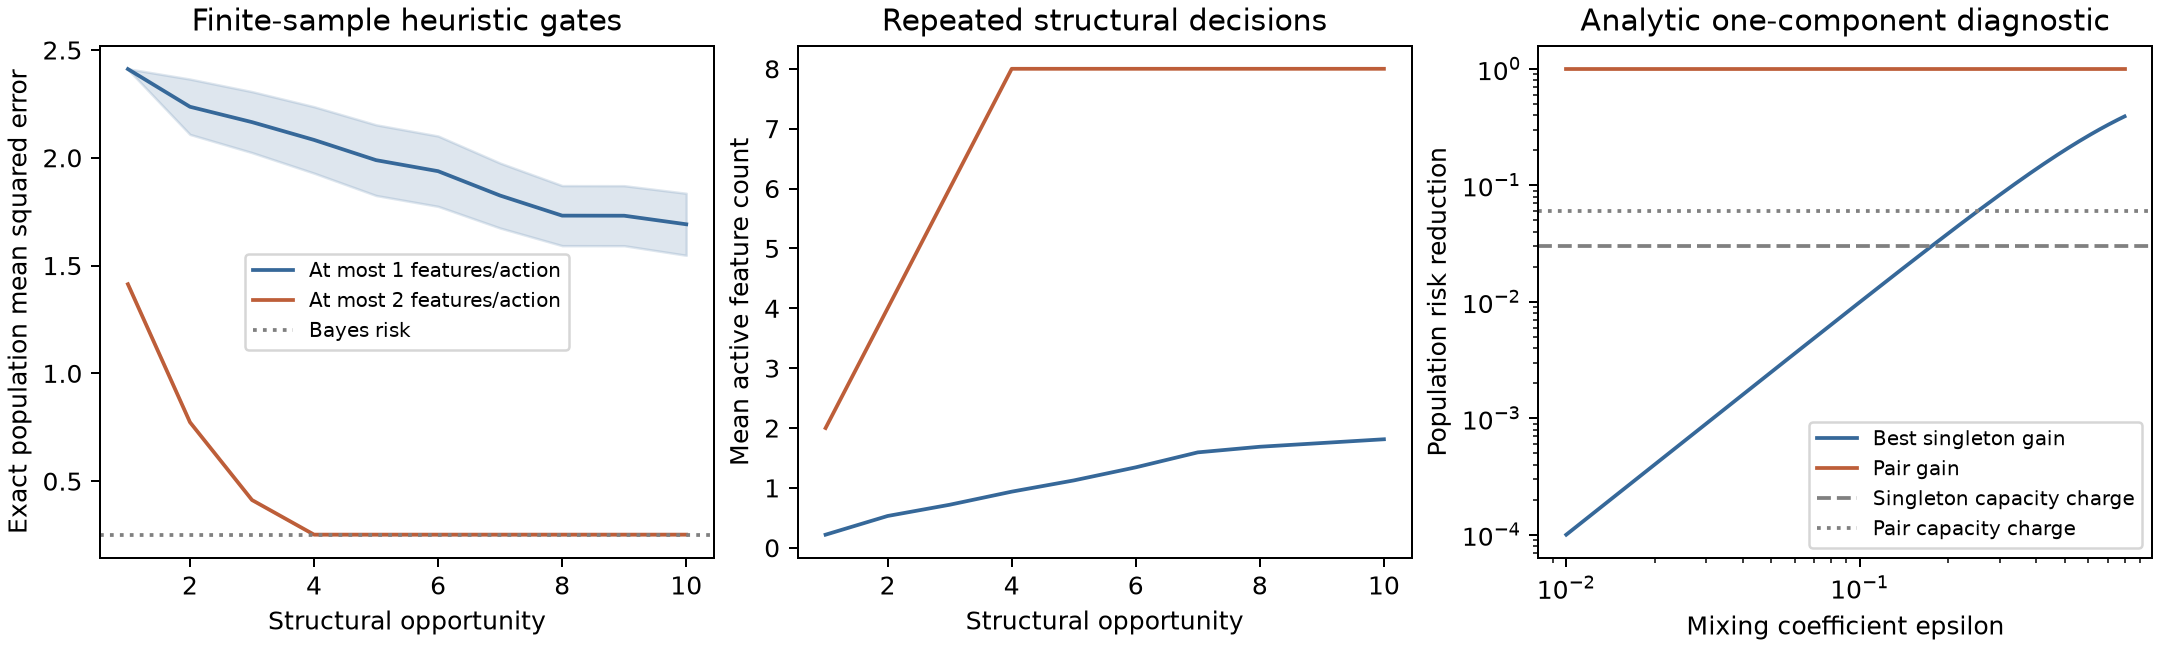
\includegraphics[width=\linewidth]{complementarity_diagnostic.png}
\caption{Auxiliary frozen-feature/readout experiment, separate from neural
hidden-parameter training. Analytic one-component quantities and measured
repeated trajectories are labelled separately. Bands are pointwise 95\%
Student-$t$ intervals over 32 independent runs; the exact population evaluator
does not enter selection. Pair enumeration
uses more candidate fits and may require large cancelling output coefficients.}
\end{figure}

\clearpage
\bibliographystyle{plainnat}
\bibliography{references}
\end{document}
